\subsection{Diseño del Preamplificador}

Los circuitos propuestos para esta etapa fueron extraídos del libro “Small Signad Audio Design” del autor Douglas Self.

El preamplificador mono se compone de dos etapas, que se detallarán de manera separada a continuación. Las mismas son.

\begin{itemize}
\item Control de Volumen.
\item Control de Tonos (Agudos, Medios y Graves).
\end{itemize}

Los niveles de línea en los equipos de audio de consumo son de un valor nominal de 0.3162 Volts eficaces. Debido a esto, los cálculos se realizaron en función de obtener una ganancia total de 10 dB(3 veces), de forma tal que con una entrada de línea de 0.3162 Vef se tenga una salida de 1 Vef a máximo volumen.

\subsubsection{Control de Volumen}

Para el control de Volumen se utilizó un control activo del tipo “Baxandall”, como el que se observa en la Figura~\ref{ctrl_vol}. El mismo consta de dos etapas, alrededor de cada uno de los operacionales que se aprecian en el circuito. El primero presenta una configuración de seguidor, con el objeto de adaptar impedancias entre la entrada y la segunda etapa, y el segundo es un amplificador inversor.


\begin{figure}[H]
\centering
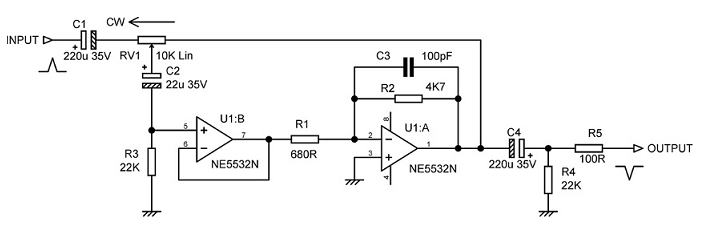
\includegraphics[width=0.55\textwidth]{img/ctrl_vol.png}
\caption{Control de volumen Baxandall.}
\label{ctrl_vol} 
\end{figure}


Por medio del potenciómetro de Control de Volumen (Rv1) se regula la proporción de la señal de entrada que será amplificada.
La máxima ganancia del sistema, igual a la máxima ganancia de la segunda etapa, será: 
$$
\vert A_v \vert = \frac{2.2 \kohm}{680 \ohm}=3.23\simeq10.2dB
$$

Los capacitores C1, C2 y C4 cumplen la función de filtros de continua, y el capacitor C3 se agrega para asegurar la estabilidad en alta frecuencia.

Para corroborar lo dicho se procedió a simular el circuito para distintos seteos del potenciómetro, como se observa en la Figura~\ref{ctrl_vol_cir_sim}. Los resultados(Figura~\ref{ctrl_vol_sim}) fueron los esperados dando una respuesta plana en las frecuencias de trabajo y una ganancia máxima de 10dB.

\begin{figure}[H]
\centering
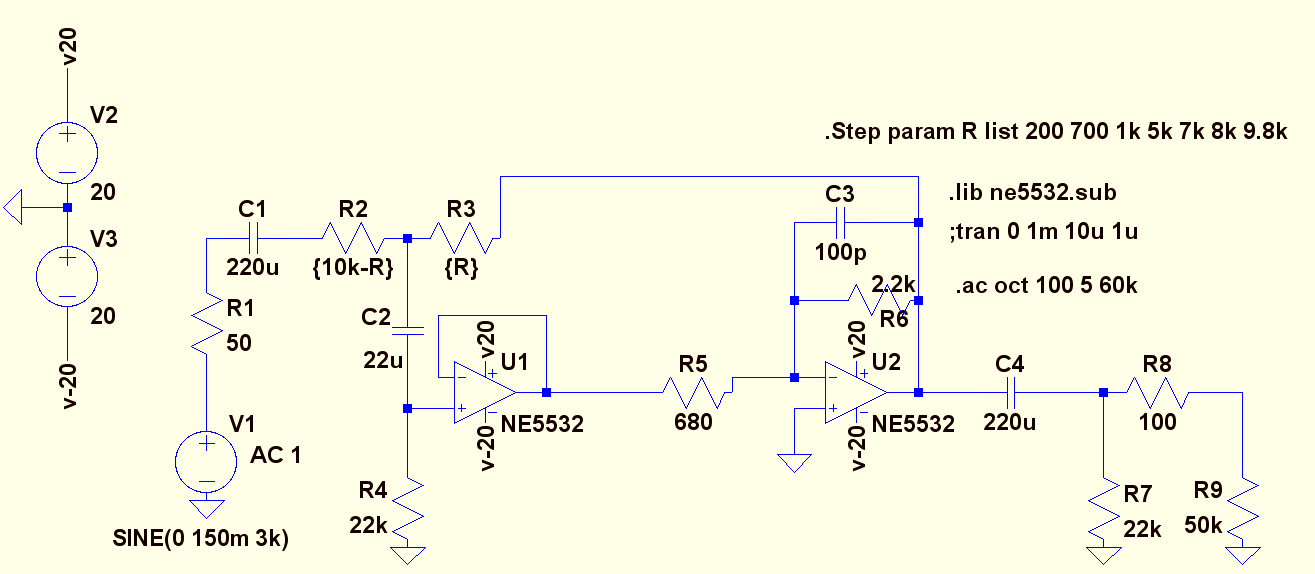
\includegraphics[width=0.75\textwidth]{img/ctrl_vol_cir_sim.png}
\caption{Circuito implementado para la simulación del control de volumen.}
\label{ctrl_vol_cir_sim} 
\end{figure}

\begin{figure}[H]
\centering
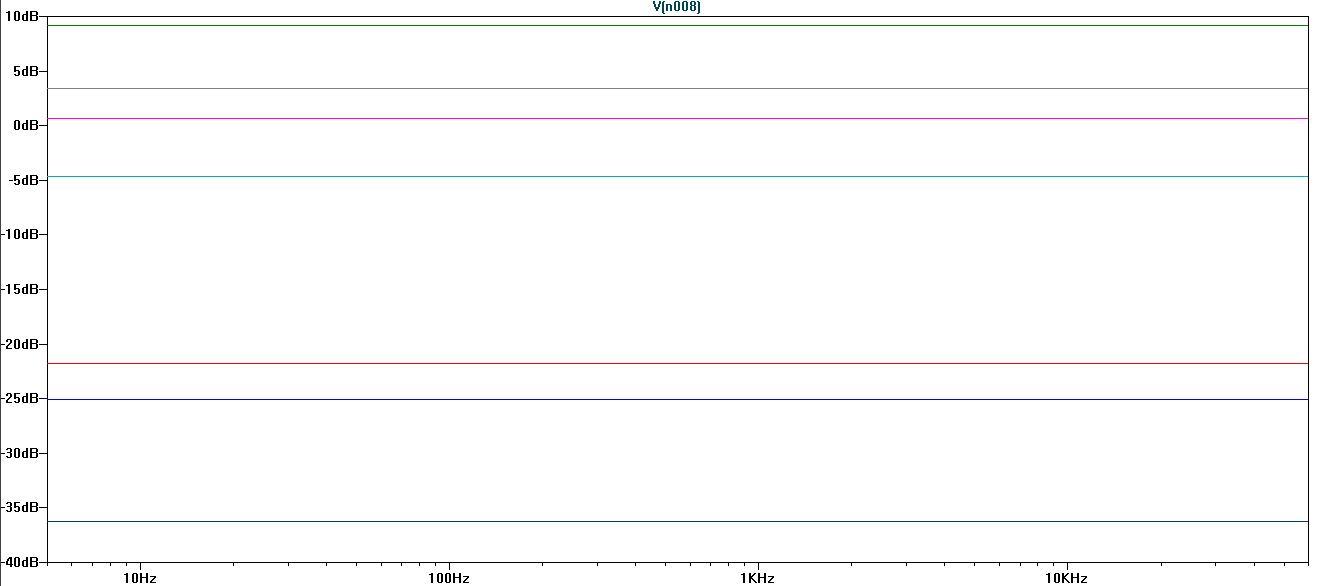
\includegraphics[width=0.75\textwidth]{img/cir_vol_sim.png}
\caption{Resultados de la simulación del control de volumen.}
\label{ctrl_vol_sim} 
\end{figure}

\subsubsection{Control de Tonos}

El circuito elegido es un control de tonos del tipo Baxandall Tribanda,  con control de agudos, medios y graves. 

El circuito funciona de la siguiente forma: 
En bajas frecuencias, el capacitor C4 se comporta como un circuito abierto, estando únicamente conectada la rama que comprende al potenciómetro RV1 (control de bajos). El mismo modifica la ganancia del operacional en configuración amplificadora de tensión para bajas frecuencias.
En medias frecuencias, el capacitor C1 se comporta como un cortocircuito, fijando para la etapa de bajos una ganancia unitaria. El capacitor C4 también permitirá el paso de la señal, mas el capacitor C3 estará aún abierto. De esta forma, por medio del potenciómetro RV2 (control de medios) se definirá la ganancia del operacional en configuración amplificadora de tensión para medias frecuencias.
En altas frecuencias el capacitor C2 también actuará como un cortocircuito, quedando tanto el control de bajos como el de medios con ganancia unitaria. El capacitor C3 se comportará como un cortocircuito, permitiendo que el potenciómetro RV3 (control de altos) defina la ganancia del operacional en configuración amplificadora de tensión para altas frecuencias.

\begin{figure}[H]
\centering
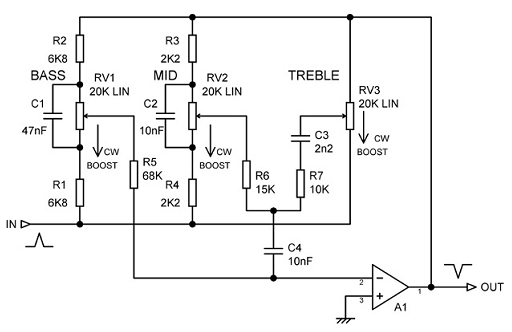
\includegraphics[width=0.55\textwidth]{img/ctrl_tonos.png}
\caption{Control de tonos Bandaxall Tribanda.}
\label{ctrl_tonos} 
\end{figure}

El esquema utilizado para la simulación se observa en la Figura~\ref{ctrl_tonos_cir} y las ganancias en dB para las variaciones de los distintos potenciómetros en la Figura~\ref{tonos_sim}.

\begin{figure}[H]
\centering
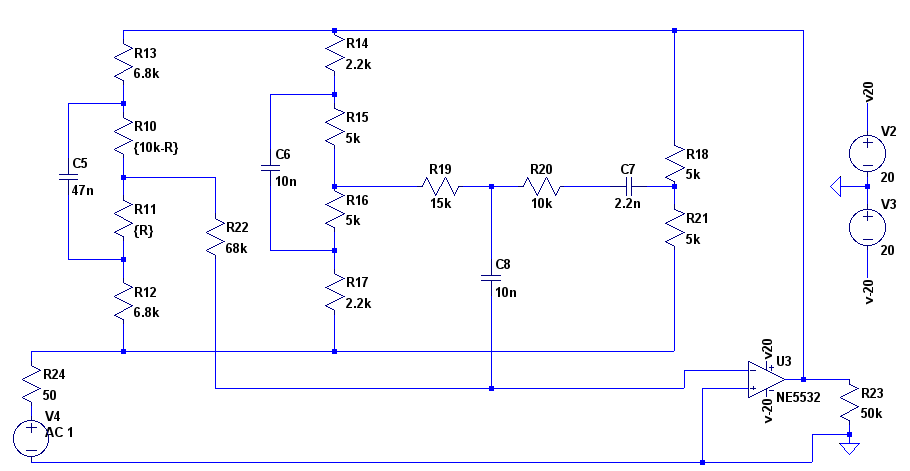
\includegraphics[width=0.75\textwidth]{img/ctrl_tonos_cir.png}
\caption{Circuito implementado para la simulación del control de tonos.}
\label{ctrl_tonos_cir} 
\end{figure}

\begin{figure}[H]
\centering
\begin{tabular}{cc}
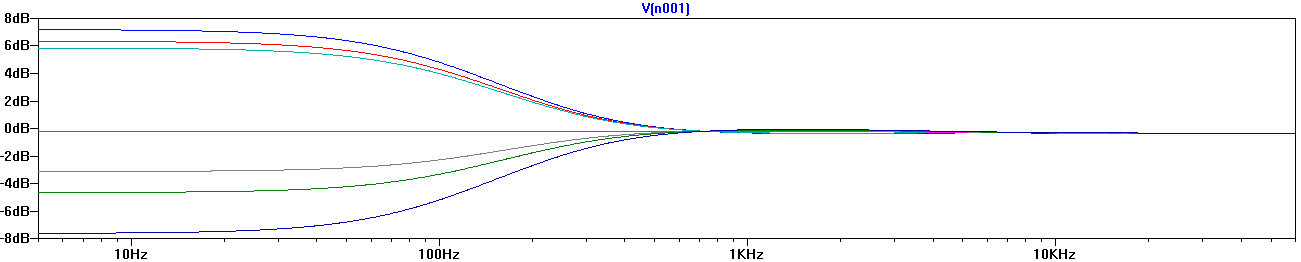
\includegraphics[width=0.75\textwidth]{img/tonos_sim_1.png}\\
\\
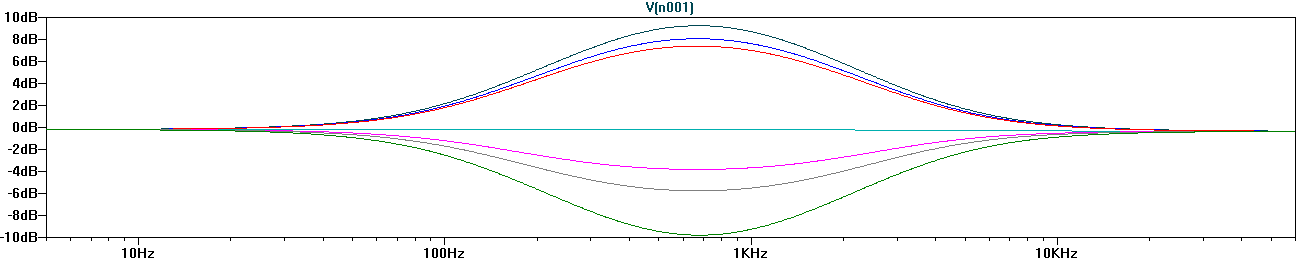
\includegraphics[width=0.75\textwidth]{img/tonos_sim_2.png}\\
\\
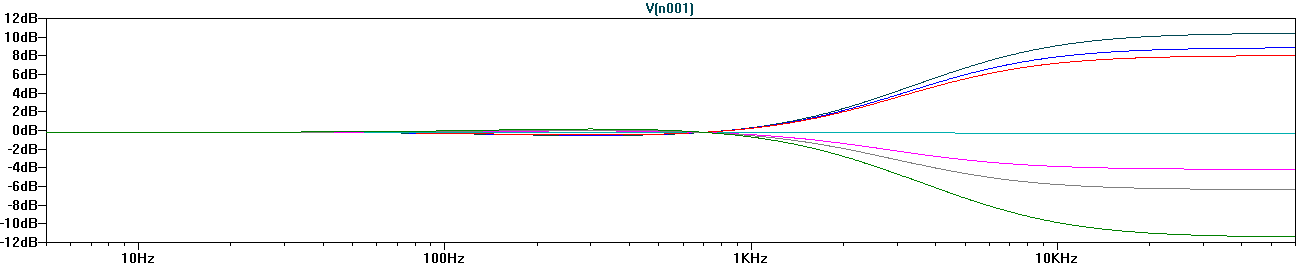
\includegraphics[width=0.75\textwidth]{img/tonos_sim_3.png}
\end{tabular}
\caption{Resultados de la simulación del control de tonos.}
\label{tonos_sim} 
\end{figure}



\medskip